%%%%%%%%%%%%%%%%%%%%%%%%%%%%%%%%%%%%%%%%%%%%%%%%%%%%%%%%
\documentclass[12pt,a4paper]{article}% 文档格式
\usepackage{ctex,hyperref}% 输出汉字
\usepackage{times}% 英文使用Times New Roman
%%%%%%%%%%%%%%%%%%%%%%%%%%%%%%%%%%%%%%%%%%%%%%%%%%%%%%%%
\title{\fontsize{18pt}{27pt}\selectfont% 小四字号,1.5倍行距
{\heiti% 黑体
计算物理Hw9报告文档}}% 题目
%%%%%%%%%%%%%%%%%%%%%%%%%%%%%%%%%%%%%%%%%%%%%%%%%%%%%%%%
\author{\fontsize{12pt}{18pt}\selectfont% 小四字号,1.5倍行距
{\fangsong% 仿宋
白博臣}\\% 标题栏脚注
\fontsize{10.5pt}{15.75pt}\selectfont% 五号字号,1.5倍行距
{\fangsong% 仿宋
(四川大学~~~物理学拔尖计划)}}% 作者单位,“~”表示空格
%%%%%%%%%%%%%%%%%%%%%%%%%%%%%%%%%%%%%%%%%%%%%%%%%%%%%%%%
\date{}% 日期(这里避免生成日期)
%%%%%%%%%%%%%%%%%%%%%%%%%%%%%%%%%%%%%%%%%%%%%%%%%%%%%%%%
\usepackage{amsmath,amsfonts,amssymb}% 为公式输入创造条件的宏包
%%%%%%%%%%%%%%%%%%%%%%%%%%%%%%%%%%%%%%%%%%%%%%%%%%%%%%%%
\usepackage{graphicx}% 图片插入宏包
\usepackage{subfigure}% 并排子图
\usepackage{float}% 浮动环境,用于调整图片位置
\usepackage[export]{adjustbox}% 防止过宽的图片
%%%%%%%%%%%%%%%%%%%%%%%%%%%%%%%%%%%%%%%%%%%%%%%%%%%%%%%%
\usepackage{bibentry}
\usepackage{natbib}% 以上2个为参考文献宏包
%%%%%%%%%%%%%%%%%%%%%%%%%%%%%%%%%%%%%%%%%%%%%%%%%%%%%%%%
\usepackage{abstract}% 两栏文档,一栏摘要及关键字宏包
\renewcommand{\abstracttextfont}{\fangsong}% 摘要内容字体为仿宋
\renewcommand{\abstractname}{\textbf{摘\quad 要}}% 更改摘要二字的样式
%%%%%%%%%%%%%%%%%%%%%%%%%%%%%%%%%%%%%%%%%%%%%%%%%%%%%%%%
\usepackage{xcolor}% 字体颜色宏包
\newcommand{\red}[1]{\textcolor[rgb]{1.00,0.00,0.00}{#1}}
\newcommand{\blue}[1]{\textcolor[rgb]{0.00,0.00,1.00}{#1}}
\newcommand{\green}[1]{\textcolor[rgb]{0.00,1.00,0.00}{#1}}
\newcommand{\darkblue}[1]
{\textcolor[rgb]{0.00,0.00,0.50}{#1}}
\newcommand{\darkgreen}[1]
{\textcolor[rgb]{0.00,0.37,0.00}{#1}}
\newcommand{\darkred}[1]{\textcolor[rgb]{0.60,0.00,0.00}{#1}}
\newcommand{\brown}[1]{\textcolor[rgb]{0.50,0.30,0.00}{#1}}
\newcommand{\purple}[1]{\textcolor[rgb]{0.50,0.00,0.50}{#1}}% 为使用方便而编辑的新指令
%%%%%%%%%%%%%%%%%%%%%%%%%%%%%%%%%%%%%%%%%%%%%%%%%%%%%%%%
\usepackage{url}% 超链接
\usepackage{bm}% 加粗部分公式
\usepackage{multirow}
\usepackage{booktabs}
\usepackage{epstopdf}
\usepackage{epsfig}
\usepackage{longtable}% 长表格
\usepackage{supertabular}% 跨页表格
\usepackage{algorithm}
\usepackage{algorithmic}
\usepackage{changepage}% 换页
%%%%%%%%%%%%%%%%%%%%%%%%%%%%%%%%%%%%%%%%%%%%%%%%%%%%%%%%
\usepackage{enumerate}% 短编号
\usepackage{caption}% 设置标题
\captionsetup[figure]{name=\fontsize{10pt}{15pt}\selectfont Figure}% 设置图片编号头
\captionsetup[table]{name=\fontsize{10pt}{15pt}\selectfont Table}% 设置表格编号头
%%%%%%%%%%%%%%%%%%%%%%%%%%%%%%%%%%%%%%%%%%%%%%%%%%%%%%%%
\usepackage{indentfirst}% 中文首行缩进
\usepackage[left=2.50cm,right=2.50cm,top=2.80cm,bottom=2.50cm]{geometry}% 页边距设置
\renewcommand{\baselinestretch}{1.5}% 定义行间距(1.5)
%%%%%%%%%%%%%%%%%%%%%%%%%%%%%%%%%%%%%%%%%%%%%%%%%%%%%%%%
\usepackage{fancyhdr} %设置全文页眉、页脚的格式
\pagestyle{fancy}
\hypersetup{colorlinks=true,linkcolor=black}% 去除引用红框,改变颜色


%%%%%%%%%%%%%%%%%%%%%%%%%%%%%%%%%%%%%%%%%%%%%%%%%%%%%%%%
\newtheorem{theorem}{\indent 定理}[section]
\newtheorem{lemma}[theorem]{\indent 引理}
\newtheorem{proposition}[theorem]{\indent 命题}
\newtheorem{corollary}[theorem]{\indent 推论}
\newtheorem{definition}{\indent 定义}[section]
\newtheorem{example}{\indent 例}[section]
\newtheorem{remark}{\indent 注}[section]
\newenvironment{solution}{\begin{proof}[\indent\bf 解]}{\end{proof}}
\renewcommand{\proofname}{\indent\bf 证明}

%%%%%%%%%%%%%%%%%%%%%%%%%%%%%%%%%%%%%%%%%%%%%%%%%%%%%%%%

\begin{document}% 以下为正文内容
    \maketitle% 产生标题,没有它无法显示标题
    %%%%%%%%%%%%%%%%%%%%%%%%%%%%%%%%%%%%%%%%%%%%%%%%%%%%%%%%
    \lhead{}% 页眉左边设为空
    \chead{}% 页眉中间设为空
    \rhead{}% 页眉右边设为空
    \lfoot{}% 页脚左边设为空
    \cfoot{\thepage}% 页脚中间显示页码
    \rfoot{}% 页脚右边设为空
    %%%%%%%%%%%%%%%%%%%%%%%%%%%%%%%%%%%%%%%%%%%%%%%%%%%%%%%%

    \begin{figure}[htbp]
        \centering
        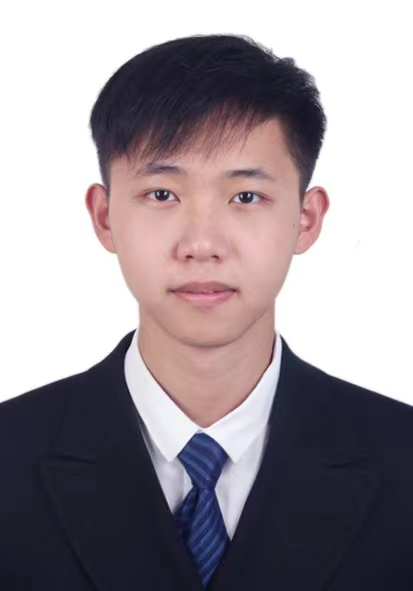
\includegraphics[height=8cm]{bbc.jpg}
        \caption{白博臣 2022141220036}
    \end{figure}

%    \begin{center}% 居中处理
%    {\textbf{Abstract}}% 英文摘要
%    \end{center}
%    \begin{adjustwidth}{1.06cm}{1.06cm}% 英文摘要内容
%        \hspace{1.5em}Attention!If you input "dif{}ferent", the computer will output "different", but if you input "dif\{\}ferent", the computer will output "dif{}ferent"
%    \end{adjustwidth}
    \newpage% 从新的一页继续


    \section{Problem 1}

    \subsection{问题回顾}
    德拜固体理论给出了温度$T$下固体的热容,其中$V$是固体的体积,$\rho$是原子的数量密度,$k_B$是玻尔兹曼常数,$\theta_D$是所谓的德拜温度,这是固体的一个特性,取决于它们的密度和声速。

    \begin{equation}
        C_V = 9V \rho k_B (\frac{T}{\theta_D})^3 \int_{0}^{\frac{\theta_D}{T}} \frac{x^4 e^x dx}{(e^x -1)^2}dx\label{eq:equation}
    \end{equation}

    固体铝组成的样品体积$V=1000 cm^3$,$\rho=6.022\times 10^{28} m^{-3}$,$\theta_D=428K$.

    我们采用辛普森方法来计算该积分,并将温度范围为$T=5K$ \ to \ $T=500K$的$C_V$的函数图像绘制出来。


    \begin{figure}[H]% 插入一张图片,H表示浮动环境下的here
        \centering
        \begin{minipage}{0.83\textwidth}% 小页面尺寸,可自行调节
            \centering
            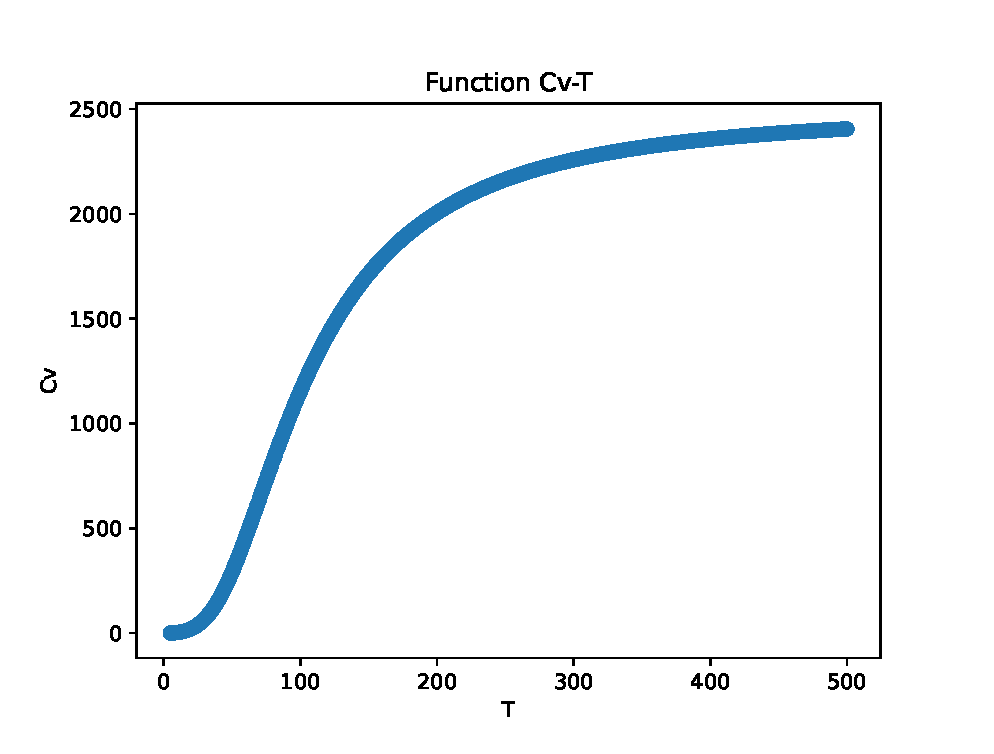
\includegraphics[width=1.0% 图片尺寸,可自行调节
            \textwidth]{Problem1}% 图片名称
            \caption{\fontsize{10pt}{15pt}\selectfont Problem1函数图像}% 图例
        \end{minipage}\label{fig:figure}
    \end{figure}


    \section{Problem 2}
    在问题二中,我们编写出了一个可以在每次二分处理前进行误差判断的自适应梯形算法与自适应辛普森算法。由题意得,当二分前后两次算法所得出的结果误差小于$\varepsilon_0 = 10^{-10}$时,停止二分并输出最终结果。

    \begin{figure}[H]% 插入一张图片,H表示浮动环境下的here
        \centering
        \begin{minipage}{0.83\textwidth}% 小页面尺寸,可自行调节
            \centering
            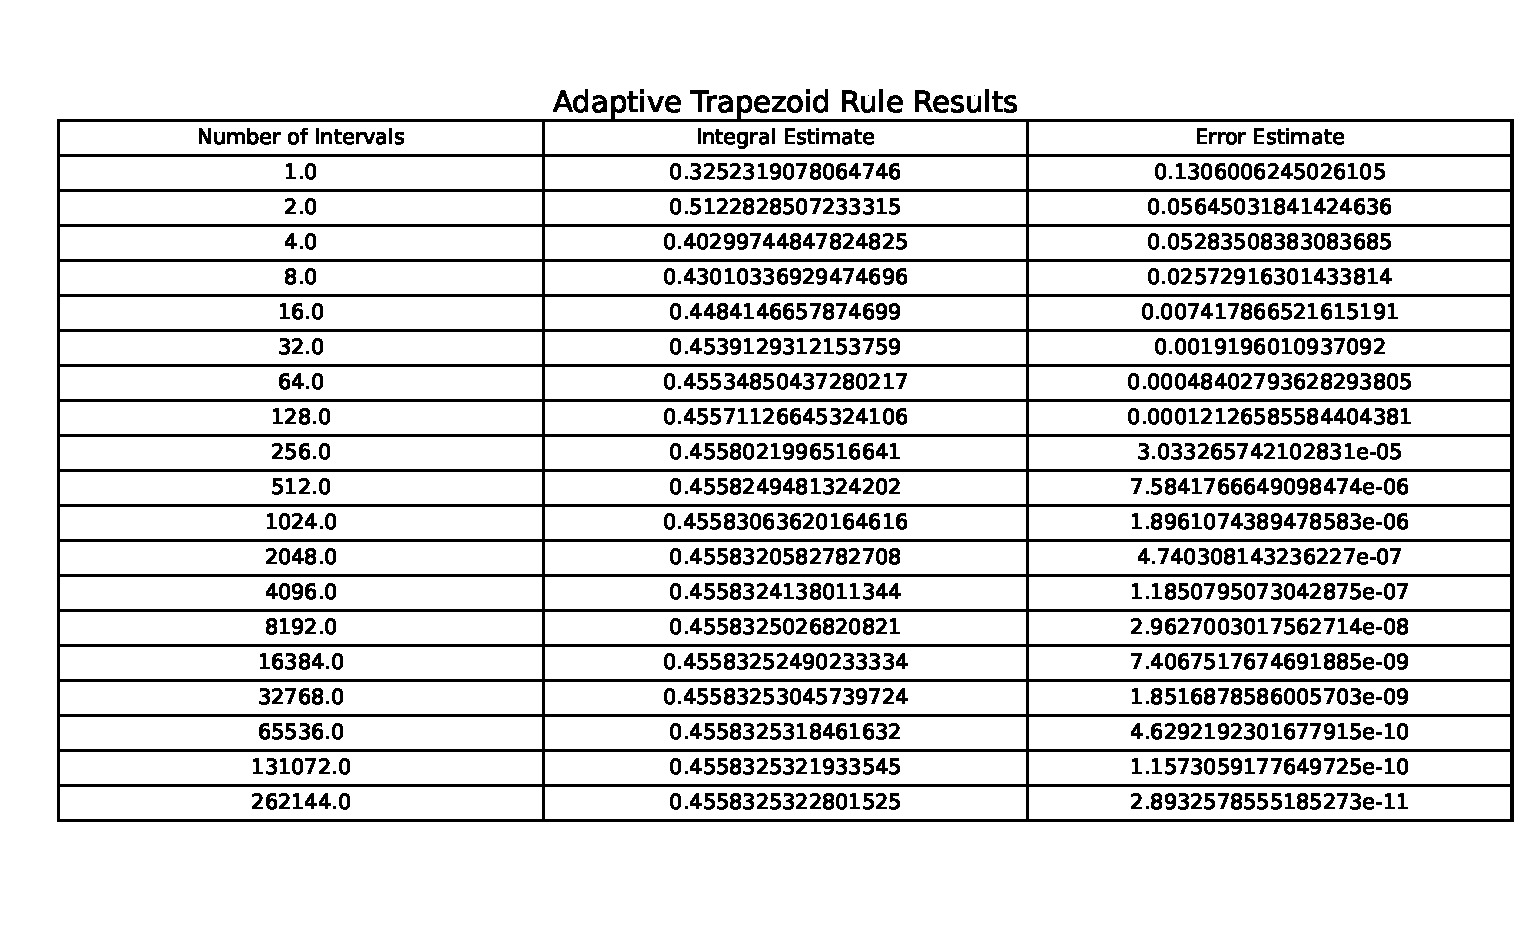
\includegraphics[width=1.0% 图片尺寸,可自行调节
            \textwidth]{Problem2.1}% 图片名称
            \caption{\fontsize{10pt}{15pt}\selectfont Problem2自适应梯形算法运算结果}% 图例
        \end{minipage}\label{fig:figure2}
    \end{figure}

    将梯形算法改为辛普森算法,再次输出运算结果:

    \begin{figure}[H]% 插入一张图片,H表示浮动环境下的here
        \centering
        \begin{minipage}{0.83\textwidth}% 小页面尺寸,可自行调节
            \centering
            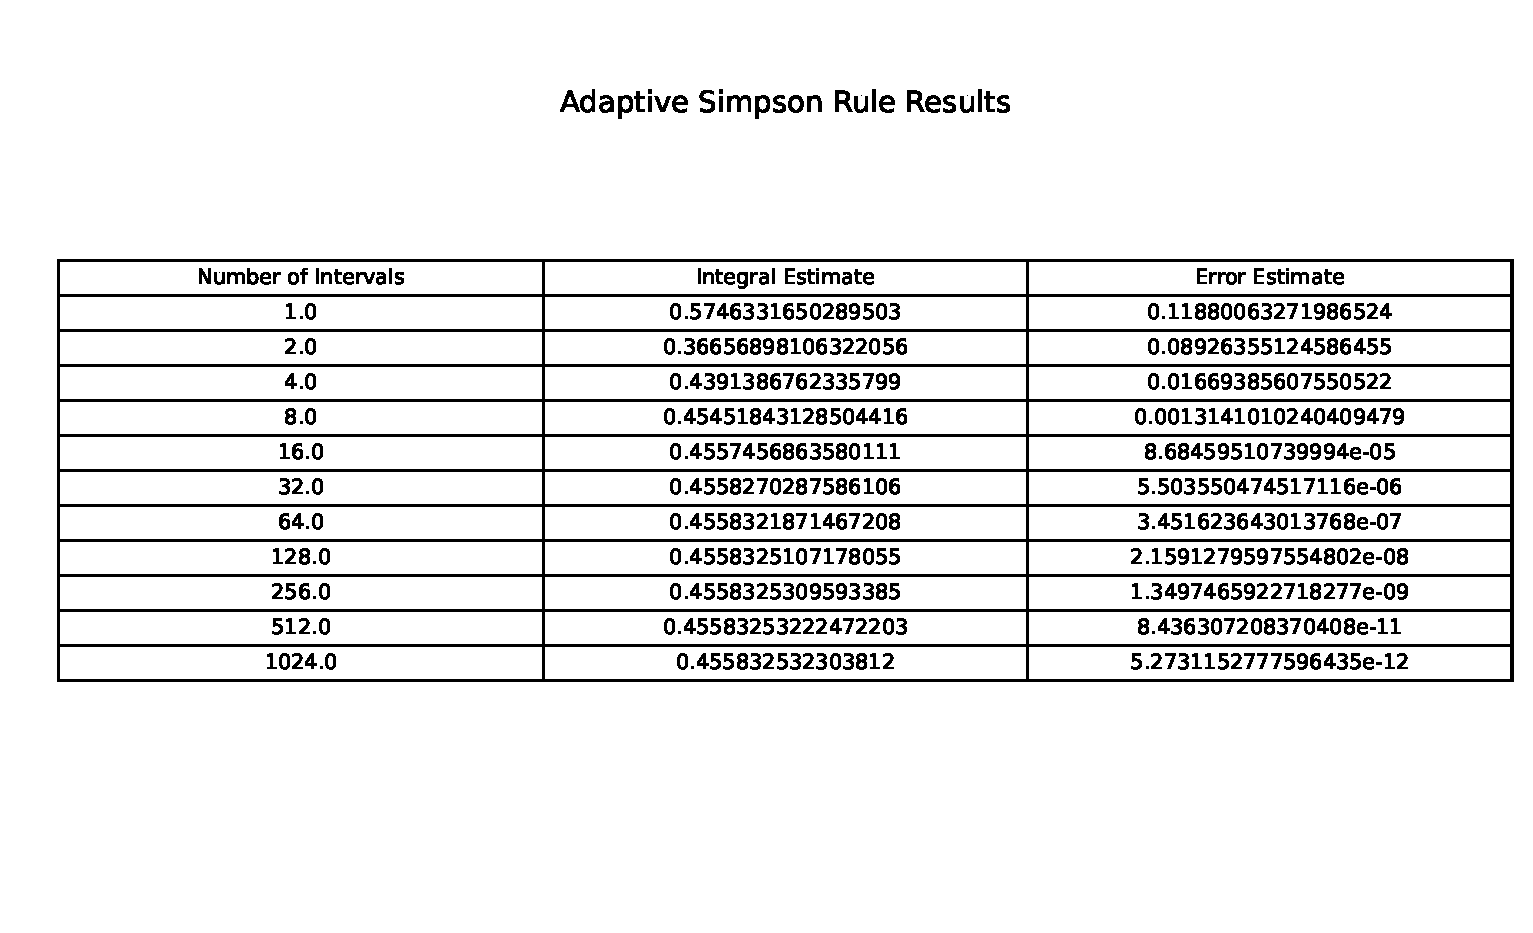
\includegraphics[width=1.0% 图片尺寸,可自行调节
            \textwidth]{Problem2.2}% 图片名称
            \caption{\fontsize{10pt}{15pt}\selectfont Problem2自适应辛普森算法运算结果}% 图例
        \end{minipage}\label{fig:figure3}
    \end{figure}

    通过表格数据我们可知,自适应辛普森算法收敛速度要明显快于自适应梯形算法,体现在收敛的所需要的n值更少。

    从原理出发,辛普森算法和梯形算法的误差估计公式如下:

    \[Simpson Error Estimated:| E_n | \leq \frac{(b-a)^5}{180n^4}\cdot K =\frac{(b-a)h^4}{180}\cdot K  \]
    \[Trapezoidal Error Estimated:| E_n | \leq \frac{(b-a)^3}{12n^2}\cdot M =\frac{(b-a)h^2}{12}\cdot M  \]

    可知实验结果与理论结果一致。h过小和过大时,误差结果偏离拟合曲线,下分析其可能的原因。
    
    1.当h较大时,$|E_n|$的高阶项部分不能忽略,仍然对结果有一定的贡献,造成了结果的偏离,当h减小时,理论上$|E_n|$应趋近于估计公式。

    2.当h逐渐减小时,由于Cancellation Error的作用,两个很接近的数字做减法,计算出的Error值不再准确,难以避免。

    \section{Problem 3}
    对于积分:$\int_{1}^{0} \frac{dx}{1+x^2} =\frac{\pi}{4} $,分别采用梯形算法、辛普森算法以及龙贝格算法进行计算,研究间隔$h$与误差大小的关系。

    对于梯形算法:

    \begin{figure}[H]% 插入一张图片,H表示浮动环境下的here
        \centering
        \begin{minipage}{0.83\textwidth}% 小页面尺寸,可自行调节
            \centering
            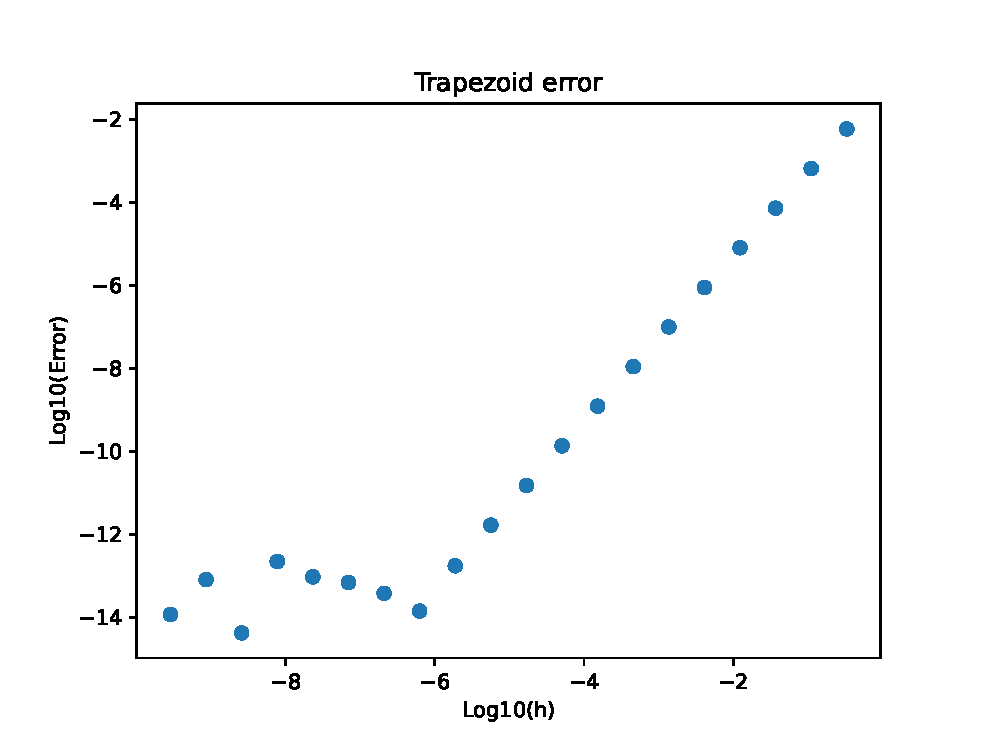
\includegraphics[width=1.0% 图片尺寸,可自行调节
            \textwidth]{Problem3.1.eps}% 图片名称
            \caption{\fontsize{10pt}{15pt}\selectfont Problem3梯形算法误差分析图}% 图例
        \end{minipage}\label{fig:figure4}
    \end{figure}

    对于辛普森算法:

    \begin{figure}[H]% 插入一张图片,H表示浮动环境下的here
        \centering
        \begin{minipage}{0.83\textwidth}% 小页面尺寸,可自行调节
            \centering
            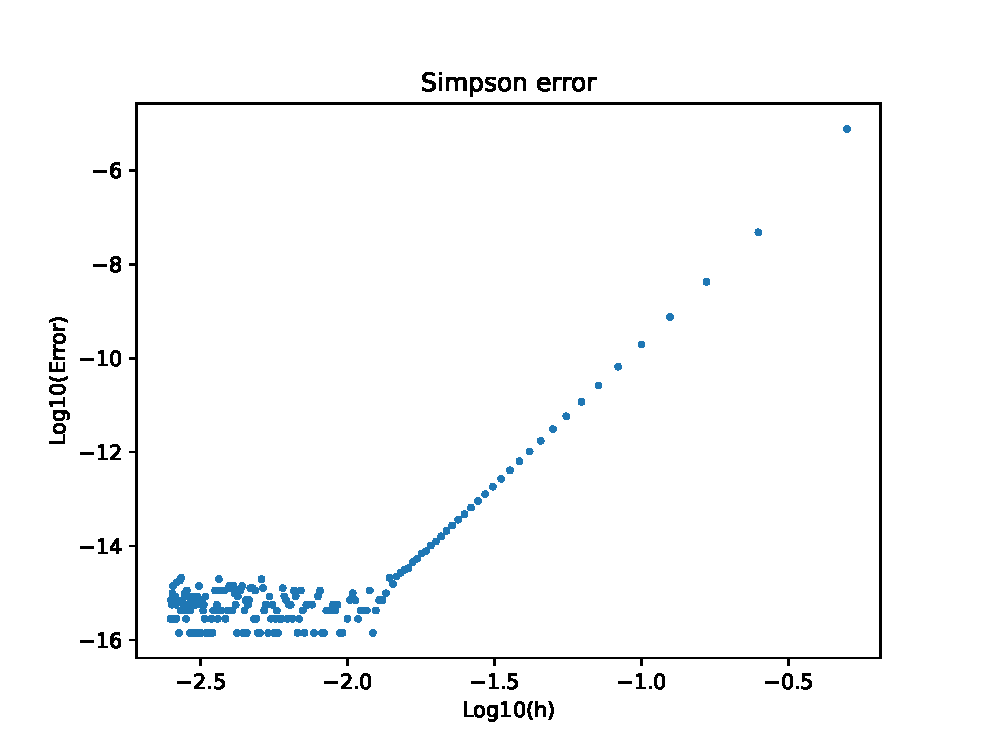
\includegraphics[width=1.0% 图片尺寸,可自行调节
            \textwidth]{Problem3.2}% 图片名称
            \caption{\fontsize{10pt}{15pt}\selectfont Problem3辛普森算法误差分析图}% 图例
        \end{minipage}\label{fig:figure4}
    \end{figure}

    对于龙贝格算法:
    \begin{figure}[H]% 插入一张图片,H表示浮动环境下的here
        \centering
        \begin{minipage}{0.83\textwidth}% 小页面尺寸,可自行调节
            \centering
            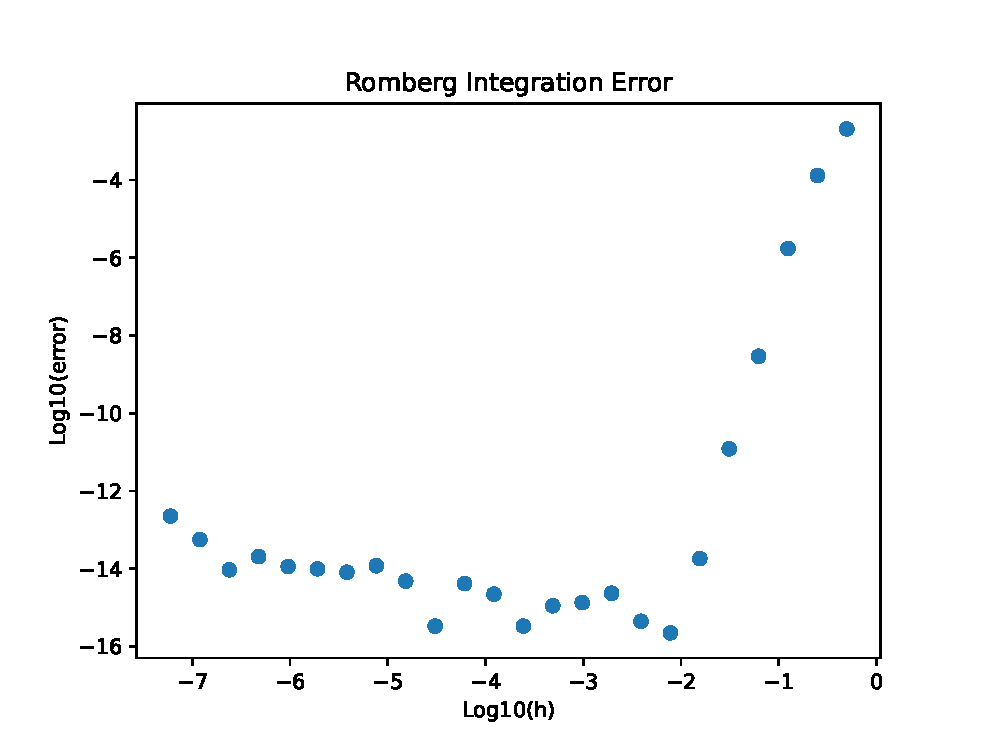
\includegraphics[width=1.0% 图片尺寸,可自行调节
            \textwidth]{Problem3.3}% 图片名称
            \caption{\fontsize{10pt}{15pt}\selectfont Problem3龙贝格算法误差分析图}% 图例
        \end{minipage}\label{fig:figure5}
    \end{figure}

    我们对图像右半部分较为平滑的部分进行斜率拟合估计如下:
    \[k(Trapezoidal) = 1.99\approx 2\]
    \[k(Simpson's) = 5.98\approx 6\]

    可知实验结果Trapezoidal方法误差与理论结果一致, Simpson's方法误差与理论结果“不一致”(理论值k(Simpson's)=4,实际值k(Simpson's)$\approx$6)。其原因解释如下:

    通过Taylor展开得到Simpson’s Rule的误差具有如下形式:
    \[|E_n| = S_1 h^4\left[f^{(3)}(a)-f^{(3)}(b)\right]+\dots\]

    当$f^{(3)} (a)-f^{(3)} (b)≠0$时,误差首项$\mathcal{O} (h^4)$起主导作用,使用Taylor中值定理得一般情况误差:$|E_n|= S_1 h^4 [f^{(4)} (ξ)],ξ∈(a,b)$,精度达到$\mathcal{O} (h^4)$。

    当$f^{(3)} (a)-f^{(3)} (b)=0$时,由Taylor中值定理得:$|E_n |=S_2 h^6 [f^{(6)} (ξ)],ξ∈(a,b)$,精度达到$\mathcal{O} (h^6)$。

    被积函数:$f(x)=\frac{1}{1+x^2}$恰好满足$f^{(3)} (1)-f^{(3)} (0)=0$,故拟合结果为$\mathcal{O} (h^6)$.

    误差拟合结果可视化如上图所示,后续偏离拟合曲线的原因可能如下:

    1.当h较大时,$|E_n|$的高阶项部分不能忽略,仍然对结果有一定的贡献,造成了结果的偏离,当h减小时,理论上$|E_n|$应趋近于估计公式。

    2.当h逐渐减小时,由于Cancellation Error的作用,两个很接近的数字做减法,计算出的Error值不再准确,难以避免。


\end{document}% 结束文档编辑,后面写啥都编译不出来
